\documentclass[11pt]{article}
% This file will be kept up-to-date at the following GitHub
%  repository: https://github.com/alexhernandezgarcia/latex-simple
%  Please file any issues/bug reports, etc. you may have at:
%  https://github.com/alexhernandezgarcia/latex-simple/issues

\usepackage{microtype} % microtypography
\usepackage{booktabs} % tables
\usepackage{url} % urls

% AMS math
\usepackage{amsmath} \usepackage{amsthm} \usepackage{amssymb}

% With no package options, the submission will be anonymized, the
%  supplemental material will be suppressed, and line numbers will be
%  added to the manuscript.  To hide the supplementary material (e.g.,
%  for the first submission deadline), use the [hidesupplement]
%  option: \usepackage[hidesupplement]{latex-simple} To compile a
%  non-anonymized camera-ready version, add the [final] option (for
%  the main track) e.g., \usepackage[final]{latex-simple} or
%  \usepackage[final, hidesupplement]{latex-simple}

\usepackage[final]{latex-simple}

% You may use any reference style as long as you are consistent
%  throughout the document. As a default we suggest author--year
%  citations; for bibtex and natbib you may use:

\usepackage{natbib}

% and for biber and biblatex you may use:

% \usepackage[% backend=biber, style=authoryear-comp, sortcites=true, natbib=true, giveninits=true, maxcitenames=2, doi=false, url=true, isbn=false, dashed=false ]{biblatex} \addbibresource{...}

\usepackage{chessboard} \usepackage{skak} \usepackage{float}
\usepackage{tikz}
\ExplSyntaxOn %requires texlive 2020, in older system load expl3
\cs_new:Npn \getfieldnumber #1 { \fp_eval:n { (\tl_tail:V #1 -1)*8 +
    \exp_args:Ne\int_from_alph:n{\tl_head:V #1} -1} } \ExplSyntaxOff

\title{GFlowChess: Joueur d'échec basé sur GFlowNet et sur Stockfish}

% The syntax for adding an author is \author[i]{\nameemail{author
%  name}{author email}} where i is an affiliation counter. Authors may
%  have multiple affiliations; e.g.:
%  \author[1,2]{\nameemail{Anonymous}{anonymous@example.com}}
\author[1]{\nameemail{Yizhan Li}{yizhan.li@umontreal.ca}}
\author[1]{\nameemail{Olivier
    Déry-Prévost}{olivier.dery-prevost@umontreal.ca}}
\author[1]{\nameemail{Sidya Galakho}{sidya.galakho@umontreal.ca}}
\author[1]{\nameemail{Simon Théorêt}{simon.theoret.1@umontreal.ca}}

% the list might continue: \author[2,3]{\nameemail{Author
%  2}{email2@example.com}} \author[3]{\nameemail{Author
%  3}{email3@example.com}} \author[4]{\nameemail{Author
%  4}{email4@example.com}}

% if you need to force a linebreak in the author list, prepend an
%  \author entry with \\:

% \author[3]{\\\nameemail{Author 5}{email5@example.com}}

% Specify corresponding affiliations after authors, referring to
%  counter used in \author:

\affil[1]{Université de Montréal}

% the list might continue: \affil[2]{Institution 2}
%  \affil[3]{Institution 3} \affil[4]{Institution 4}

% define PDF metadata, please fill in to aid in accessibility of the
%  resulting PDF
\hypersetup{%
  pdfauthor={}, % will be reset to "Anonymous" unless the "final" package option is given
  pdftitle={}, pdfsubject={}, pdfkeywords={} }

\begin{document}

\maketitle

% CCC: Contexte Contenu Conclusion

\begin{abstract}
  Les joueurs artificiels d'échec les plus performant tel que
  AlphaZero, basés sur les méthodes d'apprentissage par renforcement,
  sont en mesure de battre les meilleurs joueurs d'échecs humain.
  Dans ce rapport, nous présentons GFlowChess, un modèle génératif
  basé sur la famille de modèles GFlownet capable de simuler une
  partie d'échec suivant les règles traditionnelle du jeu à l'aide du
  jeu autonome (\textit{self-play}). Nous évaluons la performance du
  modèle à l'aide de Stockfish, un moteur d'échec moderne capable
  d'évaluer la probabilité de victoire d'une partie. Nous avons testé
  deux types de pertes ainsi que deux fonctions de récompenses pour
  observer le déroulement des trajectoires. Nous avons en effet été en
  mesure de constater les effets des fonctions de récompenses sur la
  distribution des trajectoires échantillonnées et de favoriser par
  l'entremise de la fonction de récompense un joueur. Nous discutons
  aussi les limitations associées au jeu autonome rencontrées durant
  l'entraînement.
\end{abstract}

\section*{Introduction}
% \subsection*{Les échecs et l'apprentissage automatique}
% TODO: À retirer?
Les échecs sont un jeu intellectuel notoirement difficile, compte tenu
du nombre important de règles, de pièces et variations possibles d'un
échiquier. En effet, le nombre de Shannon, qui représente une borne
inférieure sur le nombre de parties d'échec légales possibles, est
estimé à $10^{120}$. Malgré cette très grande complexité, d'important
moteur d'échec on été introduit au cours des deux dernières
décennies. Des moteurs d'échec, tel que Stockfish et AlphaZero, tel
que décrit dans \citet{alphazero}, on dramatiquement bouleversé la
scène professionnelle, en introduisant des joueurs artificiels
entraînés à l'aide de l'apprentissage par renforcement. Ces mêmes
modèles sont aujourd'hui les joueurs les plus performants, atteignant
des pointage \textit{elo} surhumain.

L'immense taille de l'espace de matchs possibles et l'aspect discret
et séquentiel des échecs font de la famille GFlowNet un bon candidat
pour échantillonner des parties d'échec et découvrir des stratégies
innovantes. Cependant, les modèles tels que Stockfish et AlphaZero
étant déjà extrêmement performants et capable de générer des
stratégies peu communes, nous nous sommes attardés à comprendre
comment nous pouvons influencer les comportements du modèles durant
une partie en modifiant la fonction de perte ainsi que la fonction de
récompense.

Nous avons entraîné notre modèle à l'aide de deux fonctions de pertes:
la fonction de perte \textit{Trajectory Balance Loss} introduit par
\citet{TBLoss} ainsi que \textit{Forward Looking Loss}, décrit dans
\citet{FLLoss}. Cette dernière fonction de perte à été choisie dans le
but de donner des récompenses intermédiaires au modèles durant la
construction des trajectoires. Intuitivement, cette approche
permettrait de guider plus efficacement le modèle vers une stratégie
efficace. De plus, nous avons entraîné GFlowChess avec types de
fonctions de récompenses: une fonction récompensant le modèle lorsque
les blancs sont avantagés et une autre récompensant des parties
égales. Finalement, notre fonction de récompense est dictée par le
moteur d'échec Stockfish, qui évalue l'échiquier et renvoie les
statistiques associées.

Notre entraînement avec la \textit{Forward Looking Loss} c'est avéré
infructueux: la fonction de perte n'a jamais convergé vers une perte
acceptable. Nous sommes incertain si la cause provient d'une erreur
d'implémentation ou bien des récompenses intermédiaires qui
ralentissent la convergence. Nous avons cependant été en mesure
d'entraîner avec succès GFlowChess avec la \textit{Forward Looking
  Loss} ainsi que nos deux fonctions de proxy. Nous avons observé
d'importantes variations du comportement dû au choix du proxy,
impliquant que GFlowChess est capable d'apprendre à échantillonner des
coups avantageux en fonction du proxy choisi.

\section*{Revue de la littérature}
Les GFLowNets sont une méthode d’échantillonage capable de
sélectionner des candidats diversifiés depuis une fonction de
récompense. Les méthodes GFlowNets étaient initialement présentées
comme un substitut au méthodes d’inférences amorties, telle que la
chaîne de Markov Monte Carlo (MCMC), \cite{gflownetfoundation}. Les
GFlowNet sont une famille de modèles génératifs récents, rendant la
littérature limitée. Néanmoins, l'intersection de l'apprentissage
automatique et des échecs est un domaine de recherche et
d'expérimentation actif depuis plusieurs années. Parmi le
développements les plus récents, nous pouvons compter Stockfish, le
moteur d'échec dont l'architecture est décrite dans par
\citet{stockfish}. AlphaZero, adapté aussi bien échecs qu'au jeu de
Go, est un développement récent démontrant les capacités surhumaines
des modèles de d'apprentissage automatique. Finalement, le projet Maia
Chess, développé par \citet{maia}, est application nouvelle de
l'apprentissage machine qui entraîne un modèle à jouer comme un humain
à l'aide de l'apprentissage par renforcement basé sur les commentaires
humains (RLHF).

Les certaines avancées récentes en lien avec les GFlowNets ont été
utilisés dans le rapport. Notamment l'usage de la fonction de perte
\textit{Trajectory Balance Loss}, qui se présente comme supérieure aux
fonctions précédentes dans le cas de longue trajectoire. La
\textit{Forward Looking Loss}, qui permet de calculer la récompense
aux étapes intermédiaires au lieu de calculer la récompense uniquement
à la fin de la trajectoire, a été utilisé afin de favoriser les coups
de qualité.

Quoique notre modèle est entraîné en jeu autonome dans un
environnement déterministe, des progrès ont été fait pour permettre
d'entraîner GFlowNet dans des environnements
stochastiques. \citet{stochasticflow} on notamment entraîné un modèle
GFlowNet dans un environnement stochastique, pavant la voix pour
l'entraînement d'un modèle GFlowNet contre un programme d'échec.

\section*{Résultats}

\subsection*{Librairies et ressources}
Nous avons fait principalement usage de 2 librairies:
\citet{hernandez-garcia2024} et \textit{Python Chess}. La première
librairie permet de faire abstraction du modèle GFlowNet et de ne
concevoir que l'environnement. La seconde librairie nous permet de
gérer la complexité des échecs et fournit presque tous les éléments
nécessaire à l'implémentation d'un environnement complet d'échec. De
plus, pour être en mesure d'évaluer la qualité des parties ainsi que
des coups jouer par GFlowChess, nous avons fais usage du moteur
d'échec Stockfish. Ce dernier est une variété de modèle de réseau de
neurone optimisé pour l'évaluation de jeux tels que le \textit{shogi}
et les échecs. Pour augmenter la vitesse d'entraînement, nous avons
paralléliser à l'aide du module Python \textit{multiprocessing} la
fonction de proxy.

\subsection*{Environnement et simplifications}
Nous avons modélisé l'environnement avec l'aide de l'objet
\textit{Board} de la librairie \textit{Python Chess}. Cet objet
contient tous les coups passé, le nombre de coups joués jusqu'à
présent, la position des pièces sur l'échiquier et les coups possibles
d'un côté et de l'autre. Nous avons modéliser les actions comme étant
un pair d'entier appartenant à $[0,63]^{2}$. Celà correspond à
associer à tout mouvement d'une pièce une case initiale,
potentiellement vide, ainsi qu'une case finale, pouvant être vide ou
pleine.  Cette modélisation simple nous permet d'interfacer facilement
avec l'objet \textit{Board} puisque cette notation est similaire à la
notation UCI. De plus, elle permet de représenter un échiquier sans
ambiguïté comme suit:

\begin{figure}[H]
  \centering \setchessboard{color=black,clearboard,showmover=false}
  \chessboard[ pgfstyle= {[base,at={\pgfpoint{0pt}{-0.3ex}}]text},
    text= \fontsize{1.2ex}{1.2ex}\bfseries
    \sffamily\getfieldnumber\currentwq, markboard]
  \caption{cases du tableau d'échiquier encodées en chiffres}
\end{figure}

Cette façon de modéliser les actions possibles de l'agent nous permet
de facilement masquer les actions invalides:

\begin{figure}[H]
  \centering
	\begin{subfigure}[b]{0.45\textwidth}
	  \centering \setchessboard{showmover=false}
          \chessboard[setfen=r5k1/1b1p1ppp/p7/1p1Q4/2p1r3/PP4Pq/BBP2b1P/R4R1K
            w - - 0 20, pgfstyle=border,markfields={d4,d6},
            color=blue!50, colorbackfield=c5, pgfstyle=color,
            opacity=0.5, color=red, markfield={d5}]
	  \caption{mouvements valides}
	\end{subfigure}
	\begin{subfigure}[b]{0.45\textwidth}
	  \centering \setchessboard{showmover=false}
          \chessboard[setfen=r5k1/1b1p1ppp/p7/1p6/2p1r3/PP1Q2Pq/BBP2b1P/R4R1K
            b - - 0 20, pgfstyle=border,markfields={d4,d6},
            color=blue!50, colorbackfield=c5, pgfstyle=color,
            opacity=0.5, color=red, markfield={d5}]
	  \caption{Mouvement invalide}
	\end{subfigure}
\end{figure}
Nous avons implémenter une fonction (\textit{get_{parents}})nous
permettant d'obtenir, pour un état donné, tous les états qui auraient
pu mener à ce même état. Or, pour mettre en oeuvre cette fonction,
nous avons fait une simplification concernant les roques. Les roques
sont un mouvements permettant d'échanger sur la même ligne le roi et
un tour de la même couleur. En effet, ceux-ci sont complexes à
modélisés et sont rares en pratique. De plus, nous avons limité à 20
coups la durée des parties, les rendant un plus courte que la partie
d'échec moyenne. Cette fonction \textit{get_parents} est complexe à
implémenter de par l'asymétrie des mouvements des pions.

Finalement, nous avons implémenter un \textit{FenParser}, c'est-à-dire
une transformation prenant un \textit{Board} et le transformant en un
tenseur de $N\times64\times13$, où $N$ est la taille du lot
(\textit{Batch}), 64 corresponds au 64 cases de l'échiquier et $13$
correspond au 13 pièces possibles sur une case.

\subsection*{Fonctions de perte et de récompense}
Nous avons utilisé deux fonctions de pertes pour entraîner nos
modèles: la fonction \textit{Trajectory Balance} ainsi que la fonction
\textit{Forward Looking}. De plus, nous avons fait usage de deux
fonctions de récompenses suivantes:
\begin{equation*}
  R_{1}(x) = - \mathbb{E}[X], \quad \text{où X=1 si les blancs gagne, 0 sinon},
\end{equation*} ainsi que
\begin{equation*}
  R_{2}(x) = - \frac{1}{1+10^{|c|/4}}, \quad \text{où $c$ est le score \textit{centipawn}}.
\end{equation*}Le score centipawn est une mesure de l'avantage des
blancs par rapport aux noirs. En effet, un score centipawn de -100 est
équivalent à ce que le joueur blanc perde un pion. Inversement, un
score centipawn de 100 est équivalent à ce que le joueur noir perde un
pion. La fonction de récompense $R_{1}$ devrait inciter GFlowChess à
faire gagner les blancs, alors que la fonction $R_{2}$ devrait inciter
GFlowNet à jouer un match aussi serré que possible, sans avantagé
aucun joueur.


\subsection*{Description et résultat des méthodes développées :}

%Actuellement, les méthodes suivantes ont été développées :

%\textbf{Initialisation de l'environnement :} \\
%L'environnement GFlowChess est initialisé en prenant en compte la
% position initiale du jeu
% sur %l'échiquier. Par défaut, une position traditionnelle est utilisée, avec la notation FEN suivante : \texttt{'rnbqkbnr/pppppppp/8/8/8/8/PPPPPPPP/RNBQKBNR w KQkq - 0 1'}

%\begin{figure}[H]
%\centering
%\setchessboard{showmover=false}
%\newgame
%\chessboard
%\caption{position initial du tableau d'échiquier}
%\end{figure}

%Dans la figure 1 nous avons la position initial du tableau
% d'échiquier correspondant à la notation
% FEN %suivante : \texttt{'rnbqkbnr/pppppppp/8/8/8/8/PPPPPPPP/RNBQKBNR w KQkq - 0 1'}.  Dans cette notation les rangées du tableau sont séparées par des "/", le nombre de case vide de droite %à gauche est représenté par des chiffres, les pièces blanches sont représentées par des lettres en %majuscules et les lettres ont les significations suivantes : \{'r': 'rook','n': 'knight','b': %'bishop','q': 'queen','k': 'king'\}


En adoptant l'encodage des cases de la figure 2, la reine Blanche à la
case 35 peut effectuer les actions : [34,33], [34,42] et [34,26] comme
montré dans la figure (a).  Donc l'action [34,18] est invalide donc il
serait masqué.

\textbf{Proxy pour l'analyse des positions :} La classe \texttt{Chess}
contient un proxy pour l'analyse des positions à l'aide du moteur
Stockfish. Présentement, nous calculons la valeur du proxy comme le
négatif de la probabilité de victoire du dernier joueur à jouer. Cette
probabilité est calculée par Stockfish.

\textbf{Résultats et défis :} \\
Nous avons été en mesure d'entraîner pour 5000 itérations un modèle
GFlowNet utilisant la perte TB. De plus, nous avons limité à 10 coups
la durée des séquences. La courbe de perte est présentée ci-dessous:
\begin{figure}[H]
  \centering 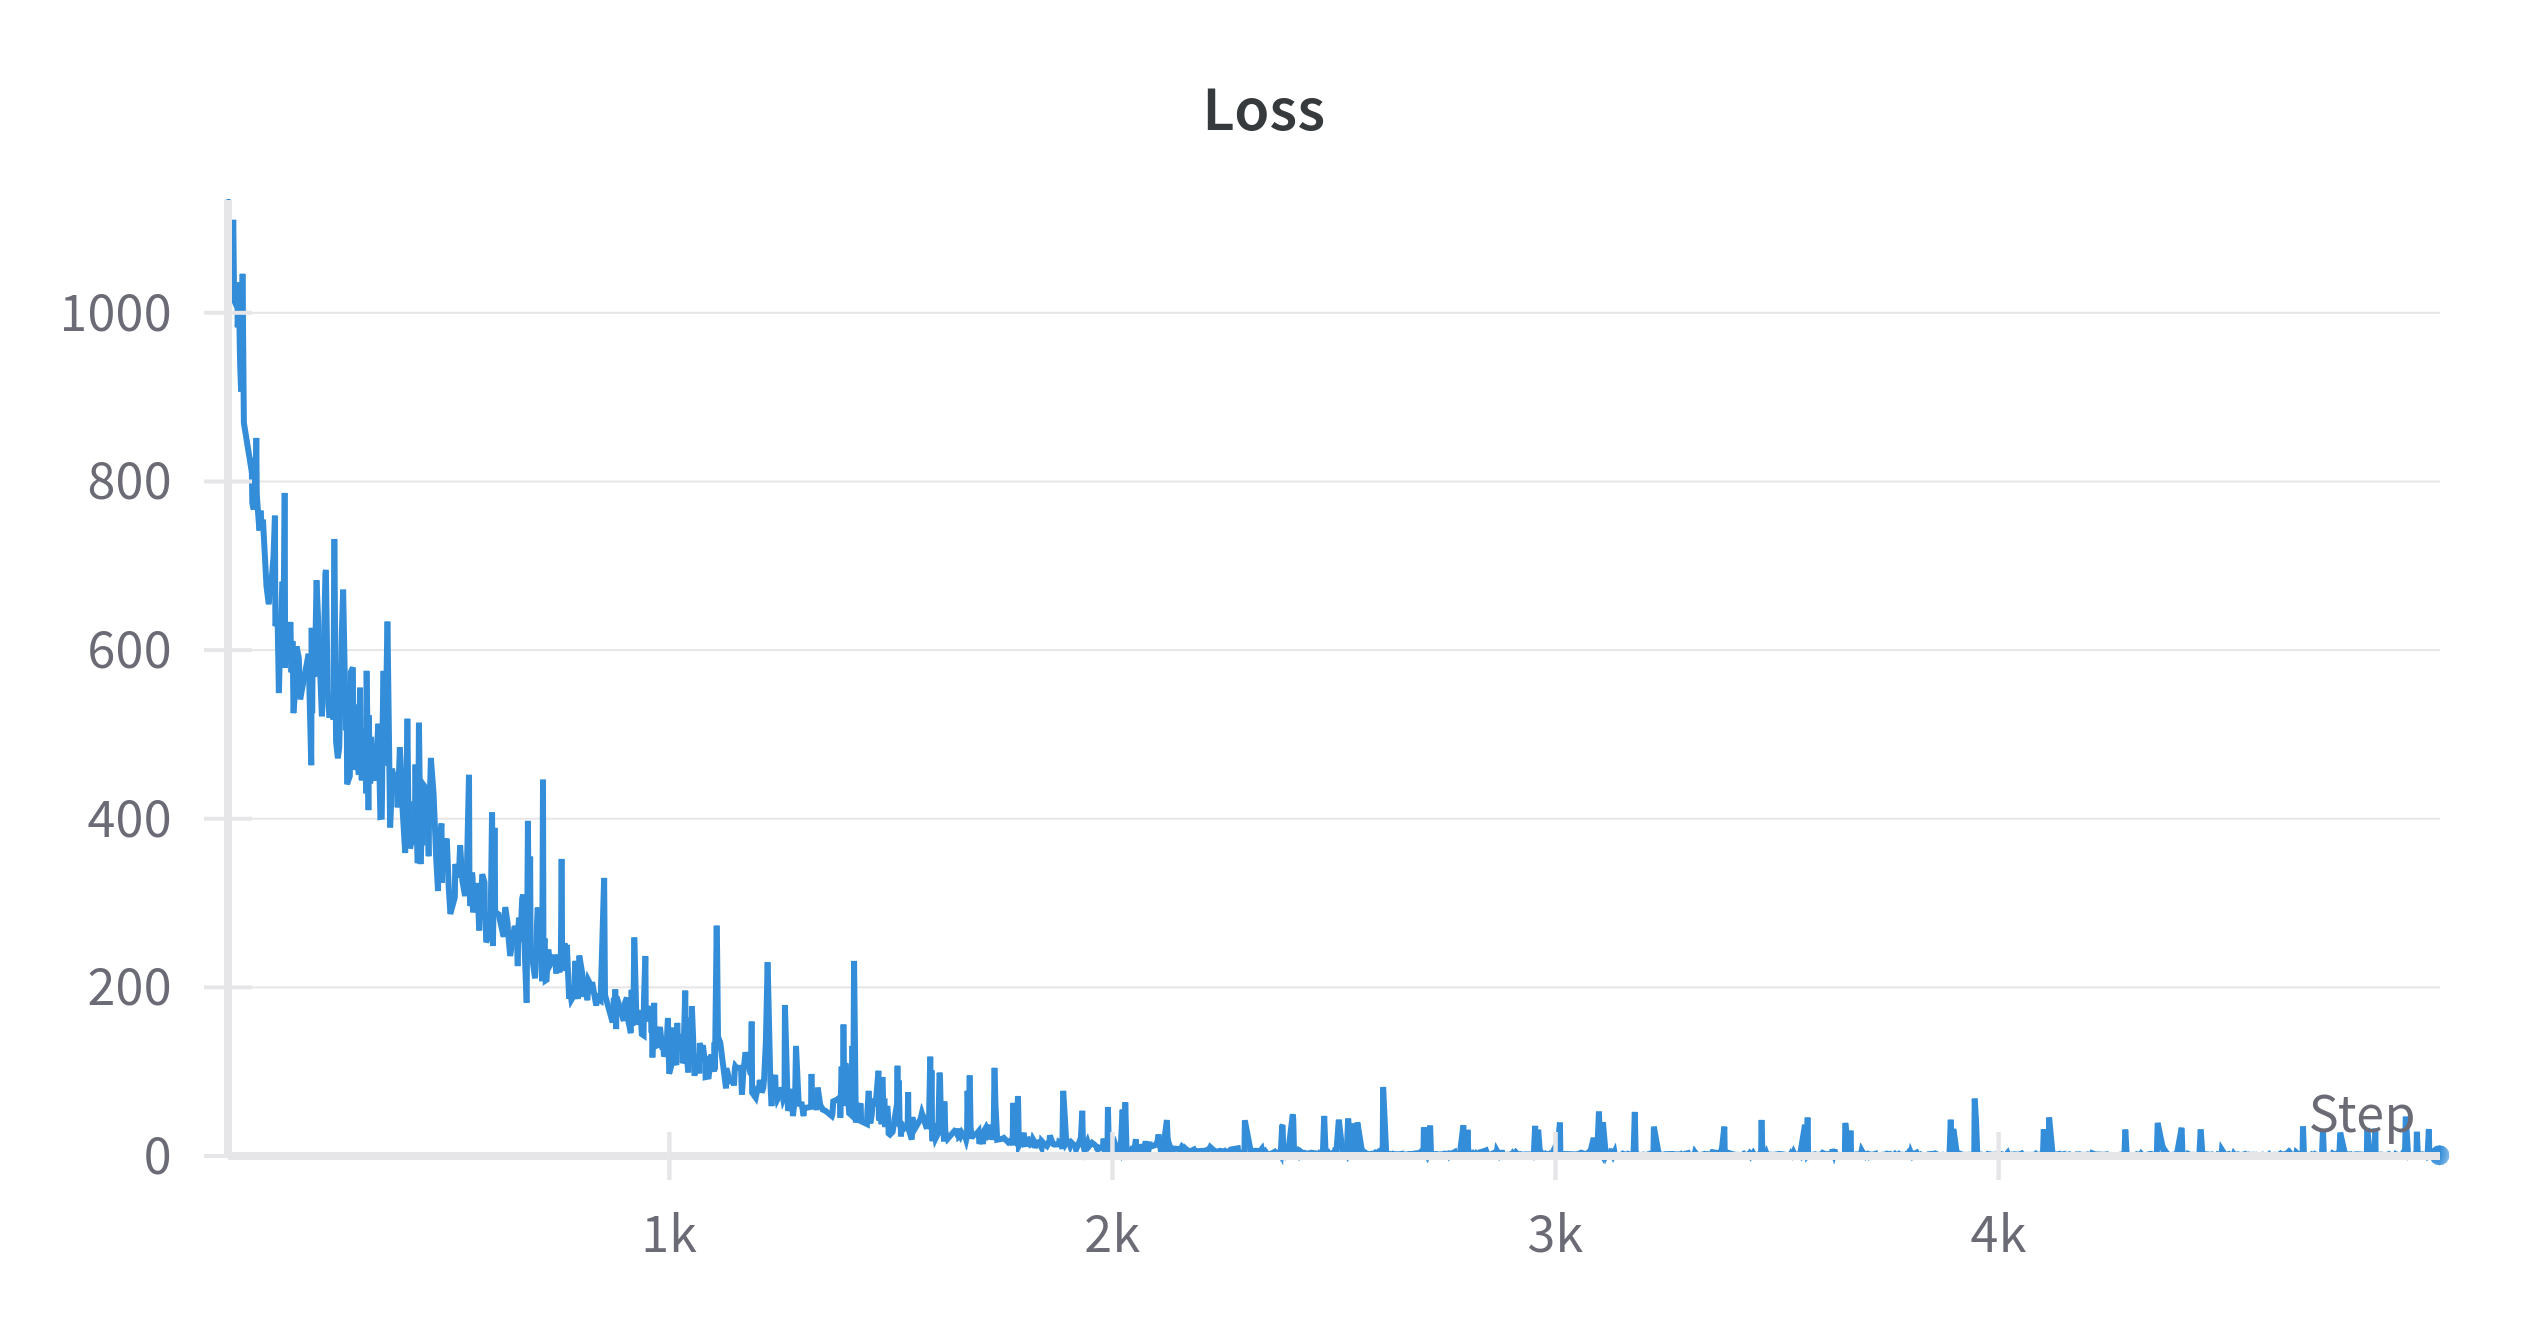
\includegraphics[scale=0.15]{tb-loss.png}
  \caption{Perte TB du modèle sur 5000 itérations}
	\label{tbloss}
\end{figure}
Or, notre modèle à encore de la difficulté à faire des ouvertures que
Stockfish juge bonne:
\begin{figure}[H]
  \centering 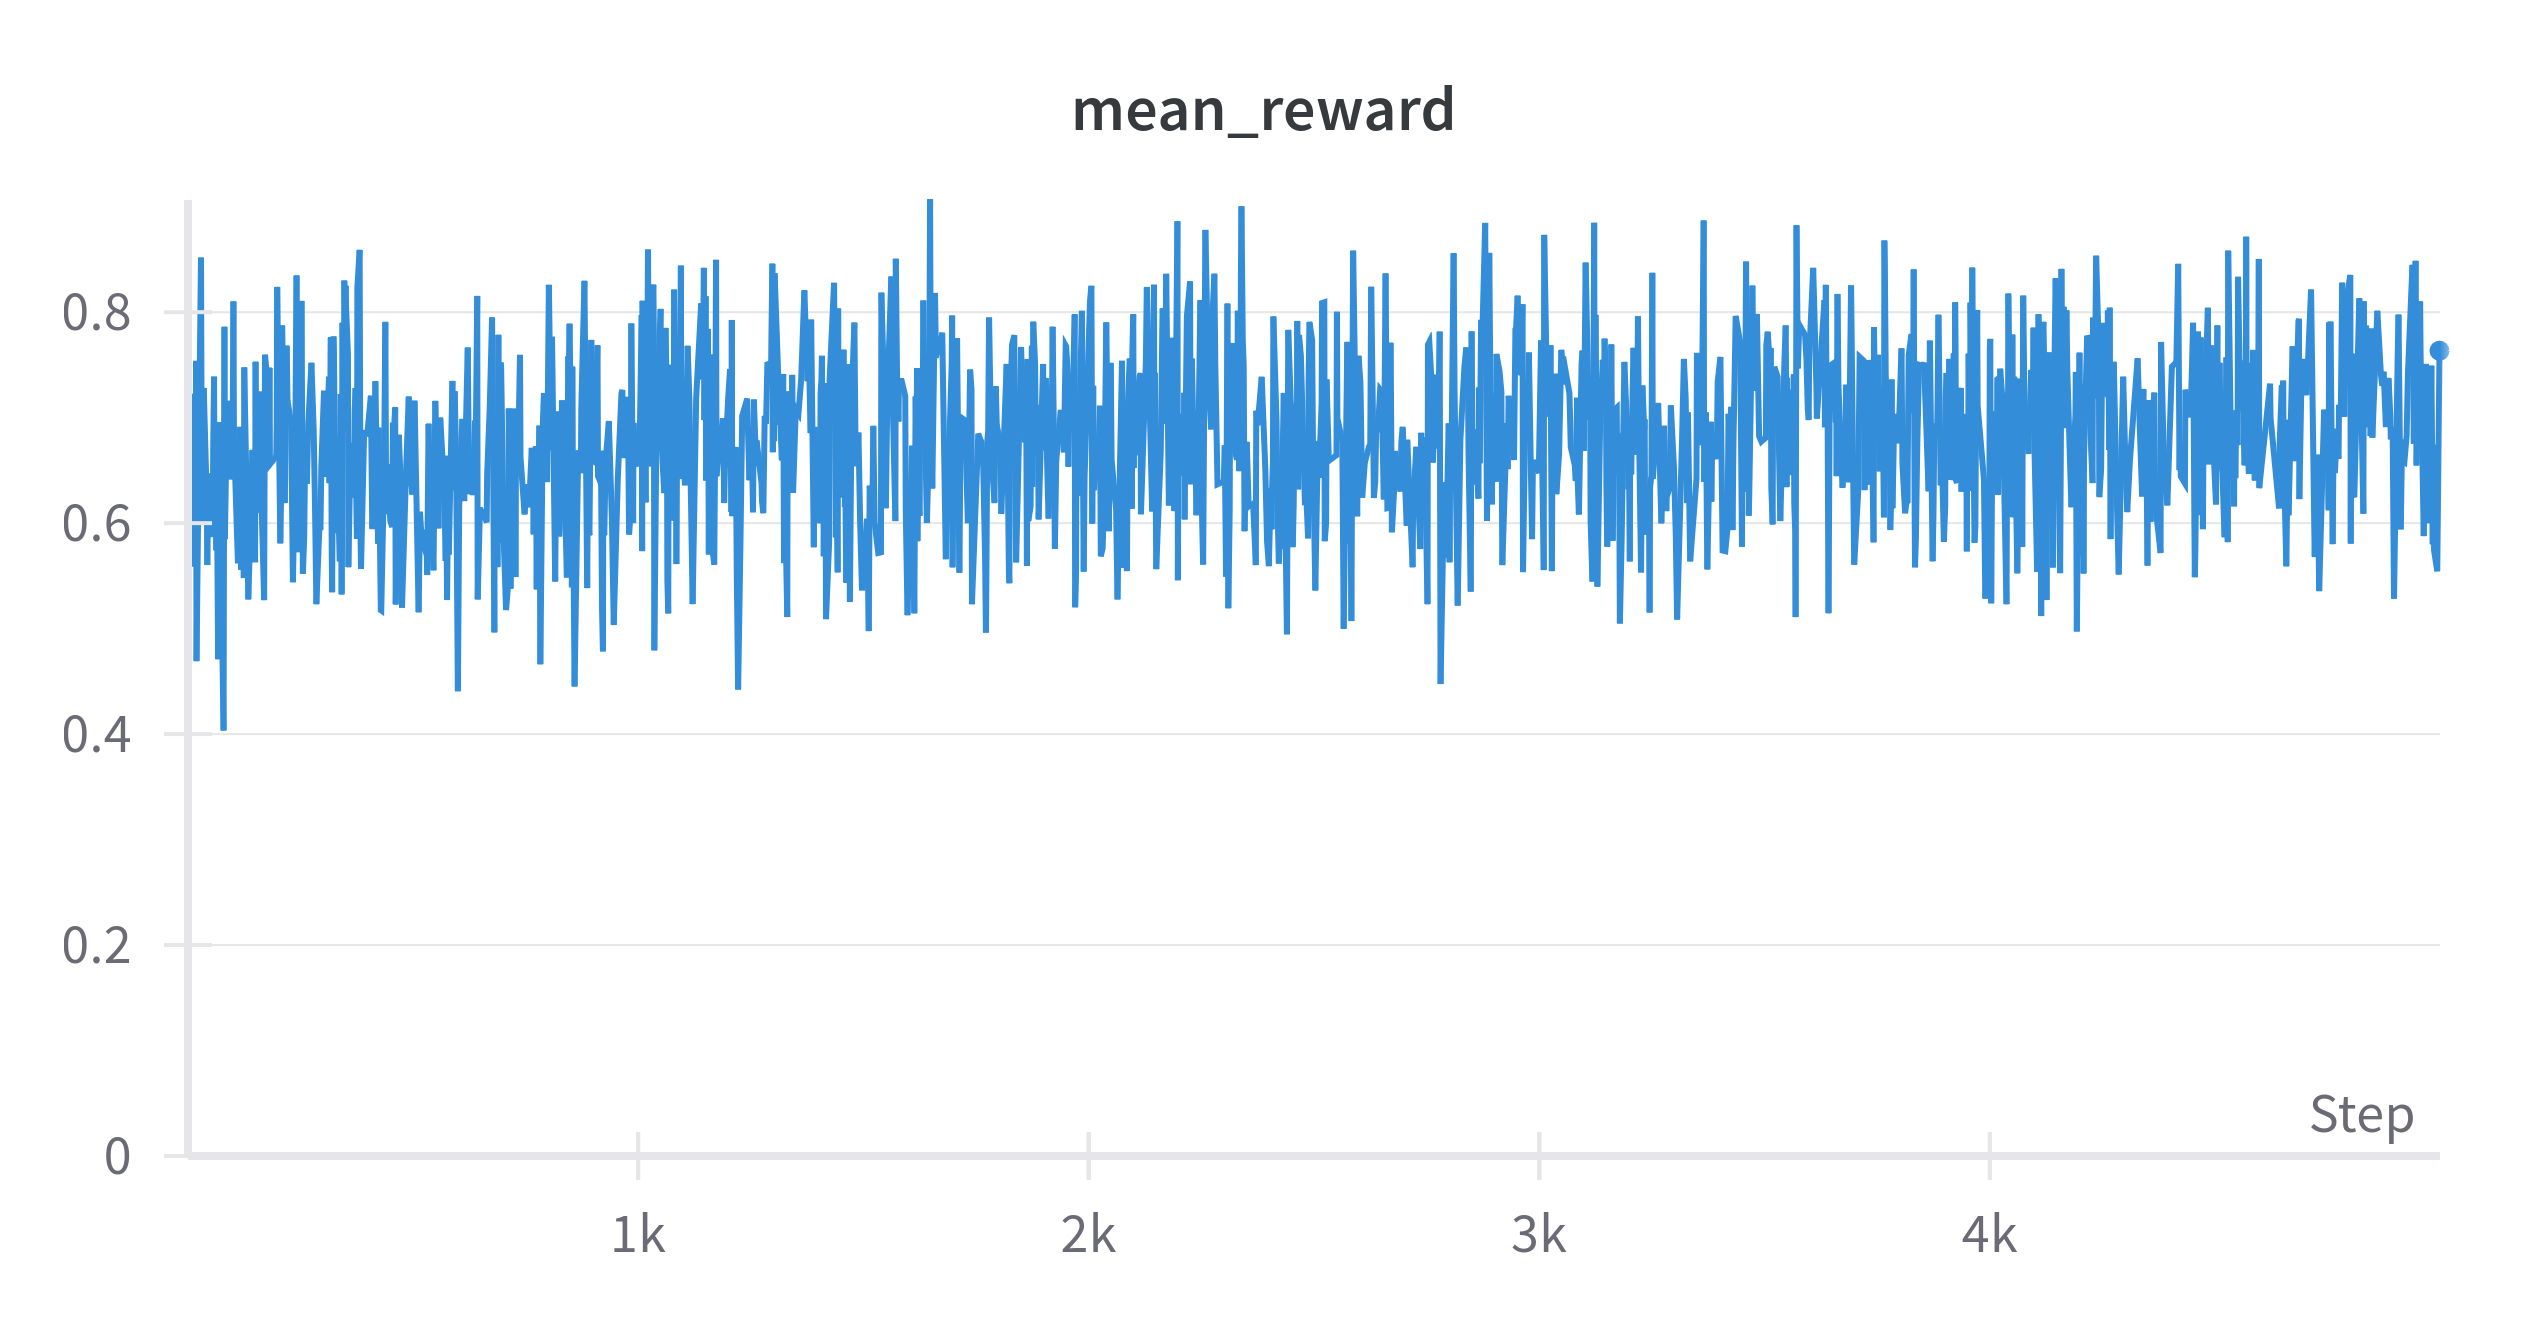
\includegraphics[scale=0.15]{tb-mean-reward.png}
  \caption{Récompense moyenne du modèle sur 5000 itérations}
	\label{tbreward}
\end{figure}
En effet, la récompense moyenne n'augmente pas durant l'apprentissage
et reste bruitée. Nous supposons que le problème est notre
\textit{proxy} actuel. En effet, notre fonction de \textit{proxy}
incite le modèle à sélectionner des coups qui avantagent le dernier
joueur à jouer (le joueur noir, dans notre cas). Au contraire, cette
fonction de \textit{proxy} incite le modèle à jouer défensivement et à
ne pas manger de pièce dès que le joueur noir à l'avantage. Une
analyse qualitative des parties échantillonnées nous pousse à croire
que cette intuition correspond à la réalité. Une fonction de
\textit{proxy} alternative consisterait à ajouter un termes positif
$\alpha d$, où $d$ représente le nombre de pièces éliminées durant une
partie et $\alpha$ correspond au poids attribué à ce terme. Ce nouveau
terme inciterait le modèle à faire des coups plus agressifs, tout en
maintenant un score Stockfish élevé.
% content will be automatically hidden during submission

% print bibliography -- for bibtex / natbib, use:


% and for biber / biblatex, use:

\bibliographystyle{latex-simple} \bibliography{references}

% supplemental material -- everything hereafter will be suppressed
%  during submission time if the hidesupplement option is provided!
\appendix

\end{document}
